In contrast to the previous project \cite{oldrepo}, no hardware design was provided. Therefore, the hardware design had to be created. The reference design \cite{TRDReferenceDesign} from Xilinx served as a template. It includes all the peripherals that are needed by the Linux kernel to run on the ZCU102 Evaluation Kit.

%\begin{figure}[htbp]
%    \centering
%    %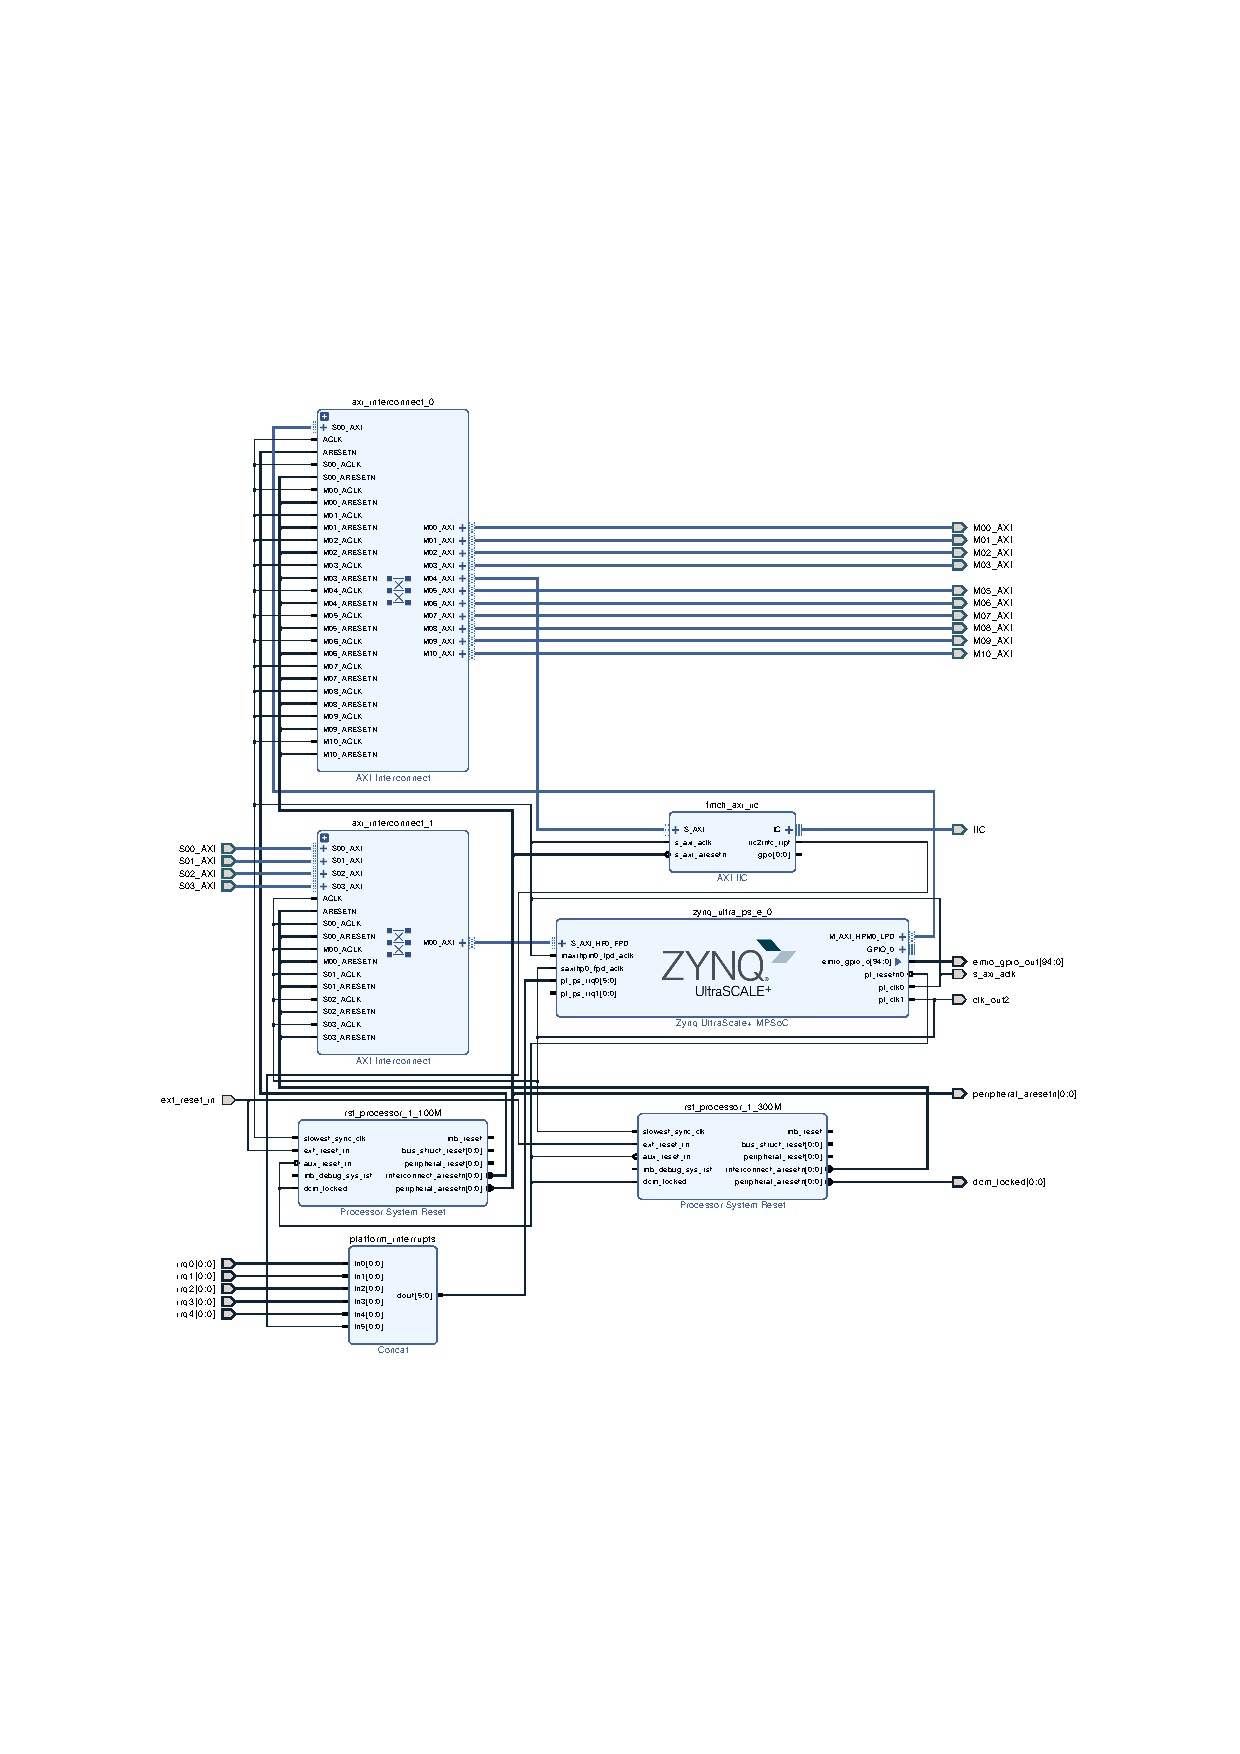
\includegraphics[width=1\textwidth, angle=0]{images/hw_design_zynq.pdf}
%    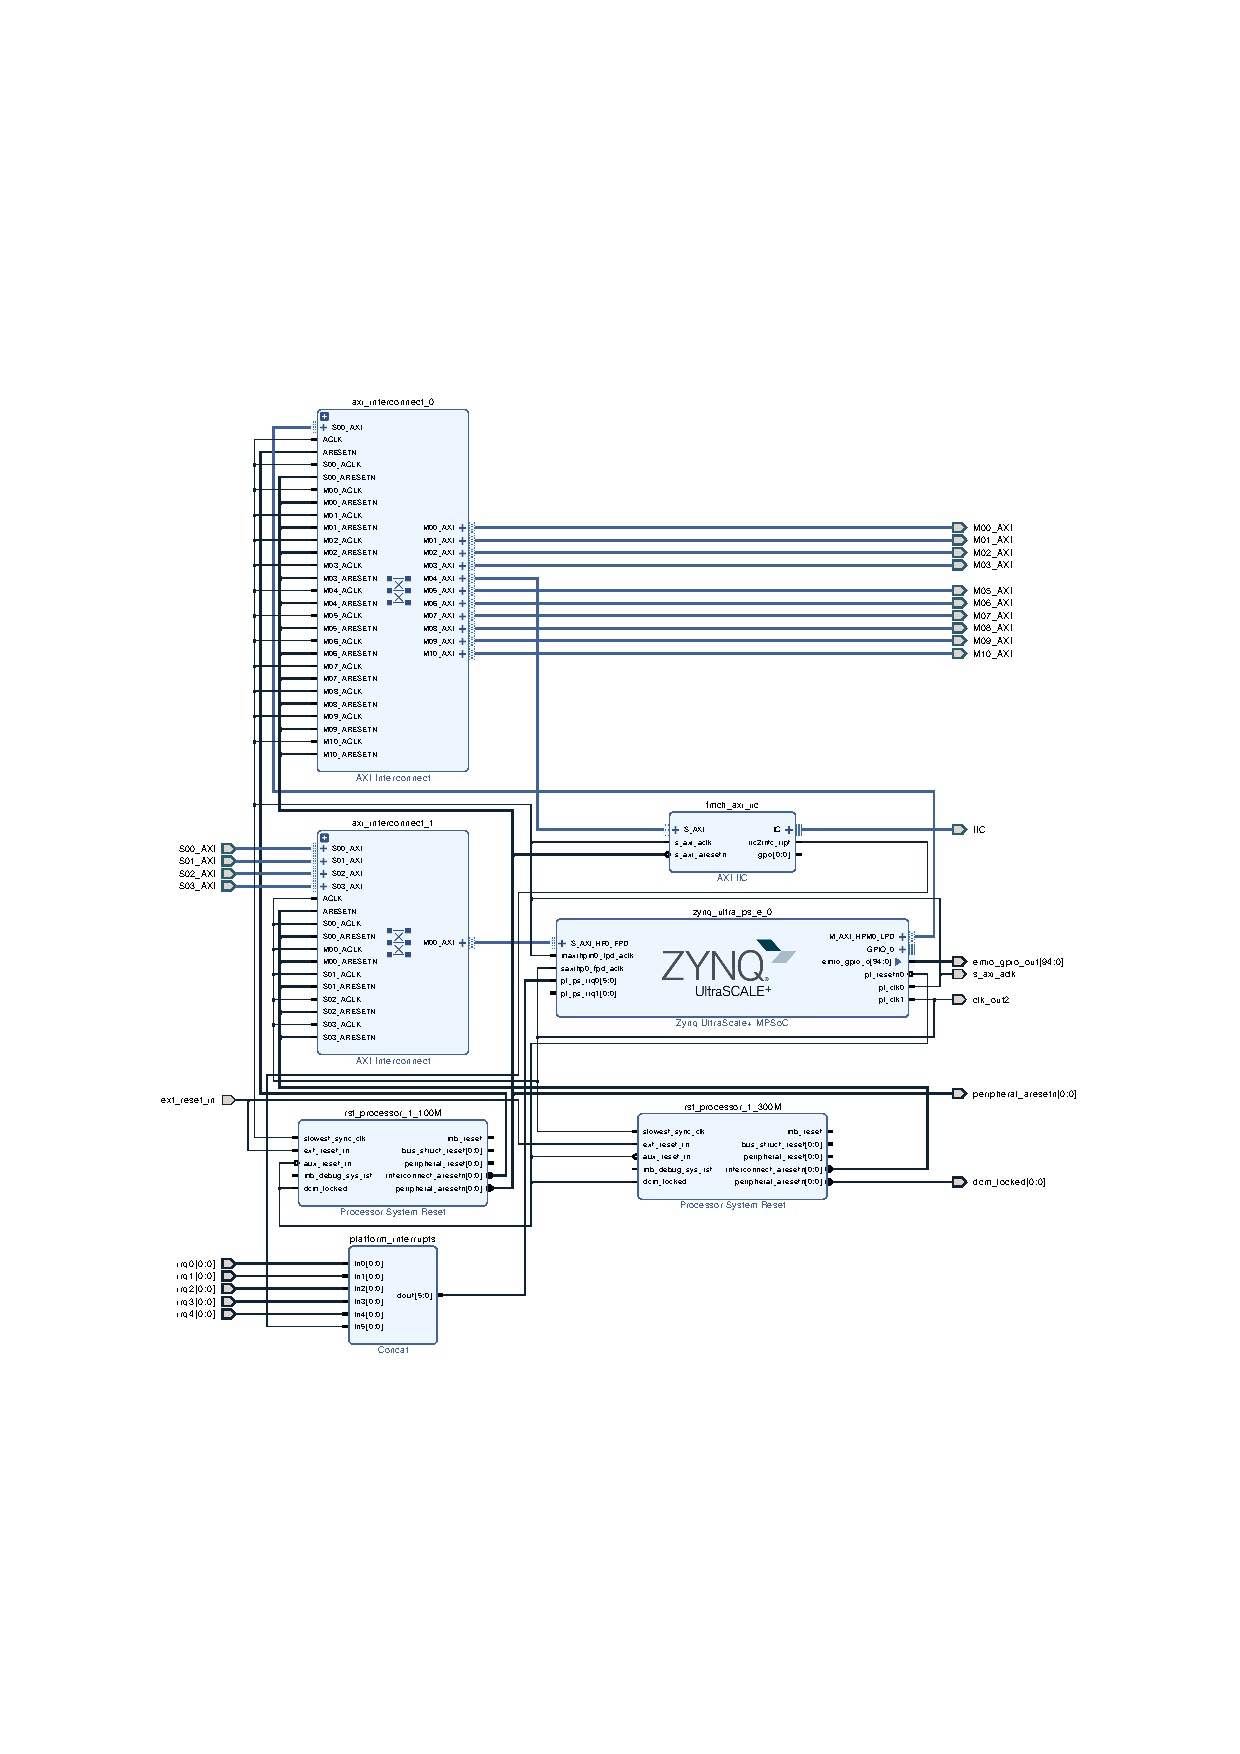
\includepdf[]{images/hw_design_zynq}
%    \caption{\label{fig:hw_zynq} Hardware design for Zynq}
%\end{figure}

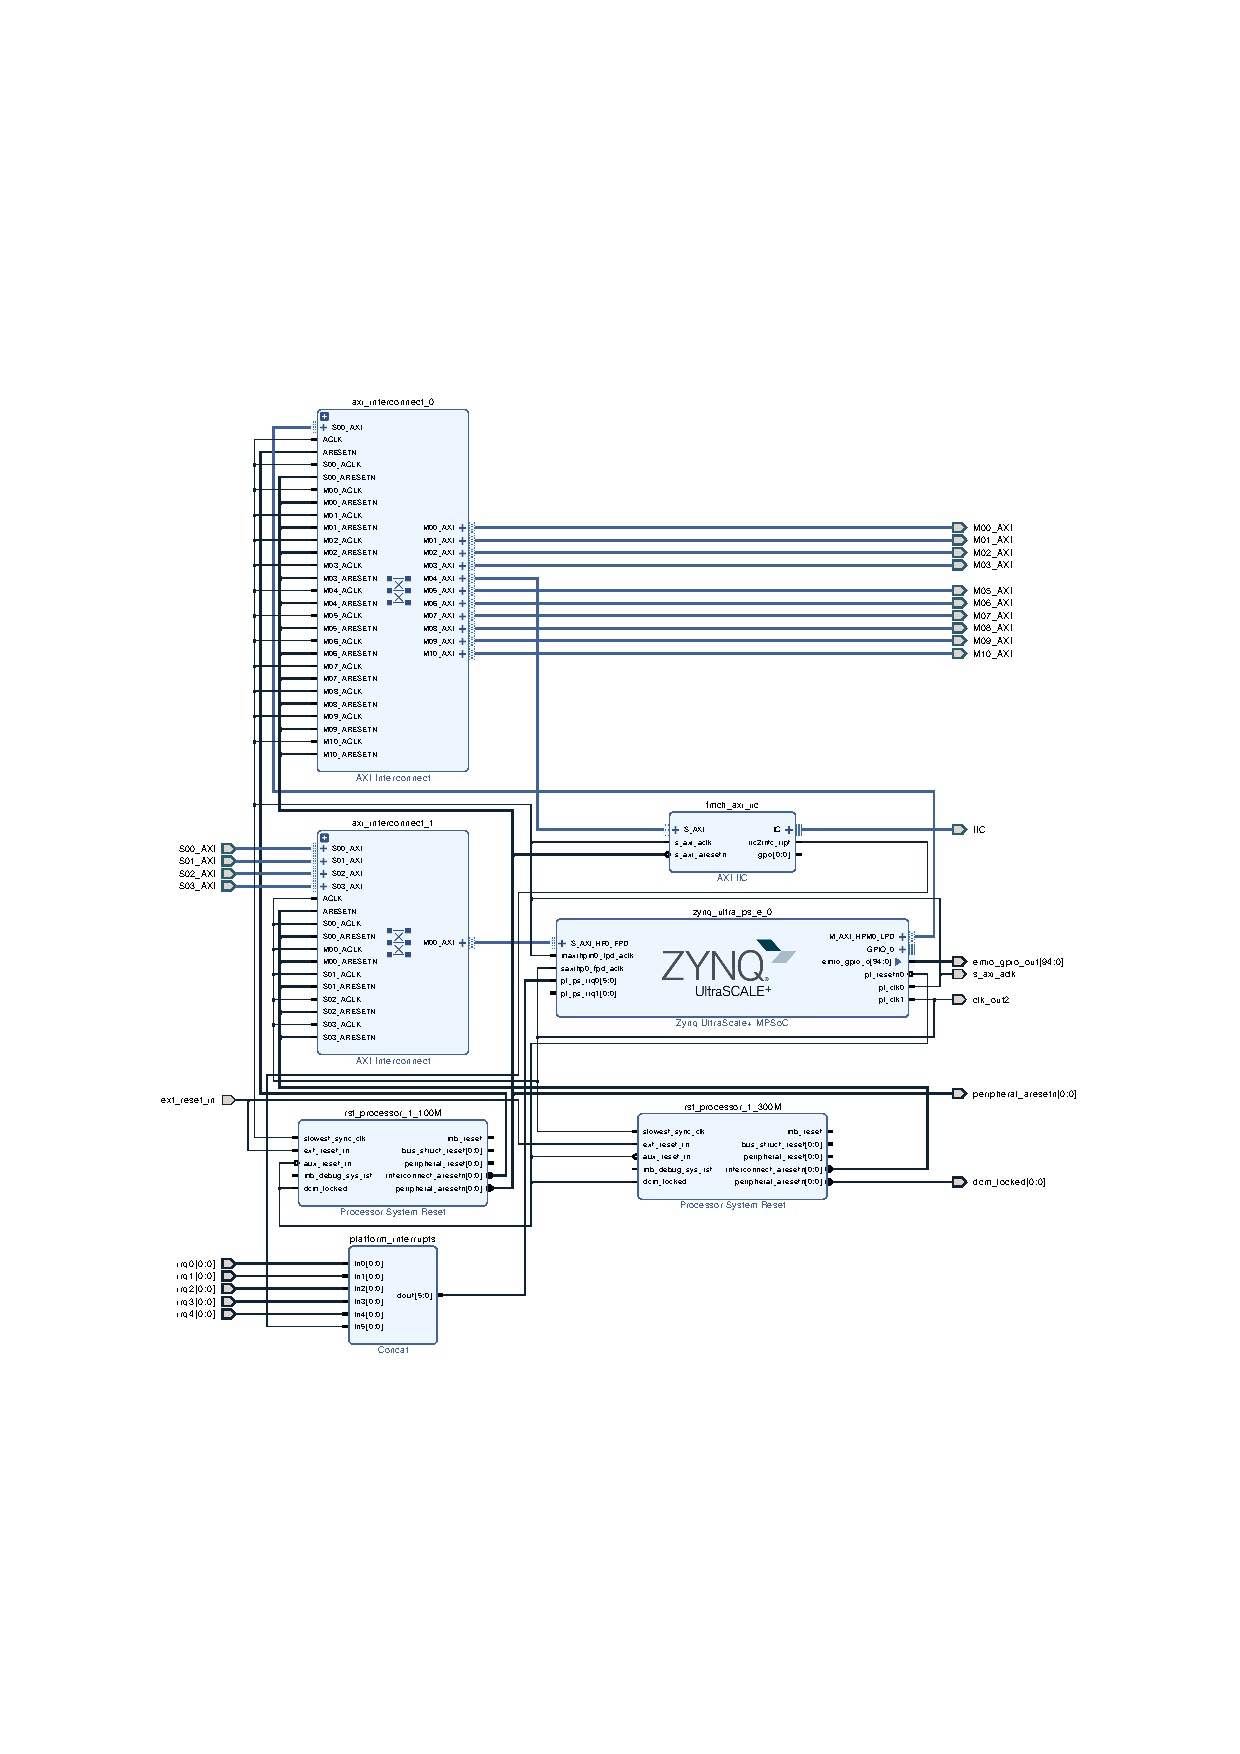
\includepdf[pages={1}]{images/hw_design_zynq.pdf}

%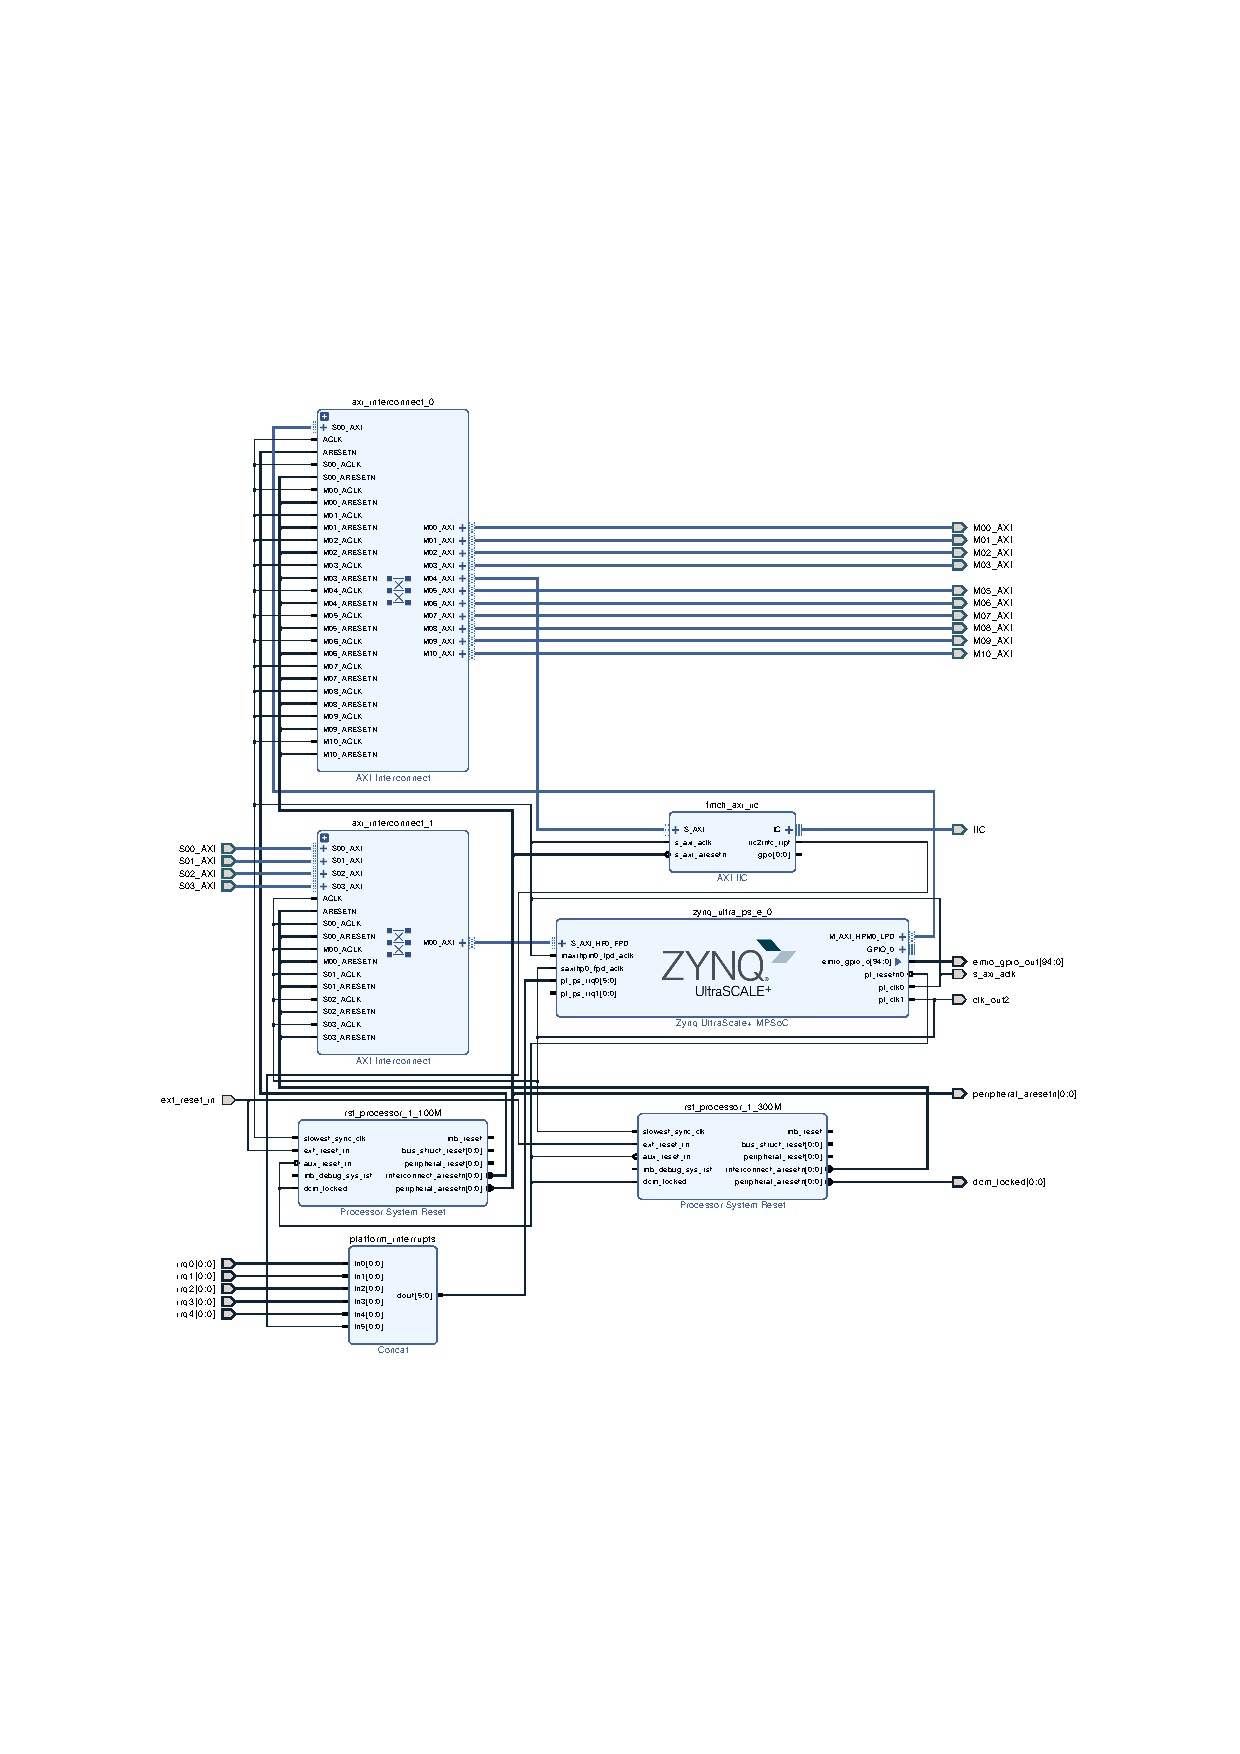
\includegraphics[]{images/hw_design_zynq.pdf}


Digilent provides a reference design~\cite{DigilentReferenceDesign} that
includes all the peripherals that are needed by the linux kernel to run on the
ZedBoard.
This is the design that is used to build the boot-image flashed onto the SD
card that comes with the ZedBoard.
It contains a \gls{xps} Project that can be opened and built using
the corresponding \emph{xps} tool that is included in the Xilinx ISE Design
Suite.
Digilent claims that they used version \emph{14.4}. Unfortunately, that version
is missing the \emph{axi\_vdma} core in revision \emph{v5\_01\_a}.
That particular revision was removed in \emph{ISE 14.4} but is available in
\emph{ISE 14.1} and replace with a newer version.
Without the knowledge of the old version, the Xilinx tools are unable to upgrade
the core to the new revision.

To mitigate this issue, both versions of \emph{ISE} were installed and the core
was imported from the old version to the new version using a symbolic link.
This allowed us to build the project in \emph{ISE 14.4}.
Since the support for \gls{dpr} is better in \emph{ISE 14.7}, we chose to use
that version.

To import the old \emph{axi\_vdma} core into the new version of \emph{ISE}, the
command in \Cref{lst:corelink} can be used, assuming \emph{ISE} was installed in
the default directory \emph{/opt}.
\begin{lstlisting}[
	language=Bash,
	caption={Link \emph{axi\_vdma} core from \emph{ISE 14.1} to \emph{14.4}},
	label={lst:corelink},
	basicstyle=\small,
	float=h,
	floatplacement=h
	]
	ln -s /opt/Xilinx/14.1/ISE_DS/EDK/hw/XilinxProcessorIPLib/pcores/axi_vdma_v5_01_a /opt/Xilinx/14.7/ISE_DS/EDK/hw/XilinxProcessorIPLib/pcores/axi_vdma_v5_01_a
\end{lstlisting}

This design can then be adapted to include our logic needed for the hardware
accelerators.
Digilent published a tutorial~\cite{DigilentTutorial} on how to do this on a
simple example.
The basic steps to do this are:
\begin{itemize}
	\item Create new peripheral by choosing `Hardware', `Create or Import
		Peripheral\ldots'
	\item The new peripheral can now be found in the `Project Local PCores'
		under the `USER' registry.
		Add it to the design by right clicking on it and choosing `Add IP'
	\item Add it to the Zynq Processing System when prompted to do so
	\item Assign an address and memory size in the `Addresses' tab
\end{itemize}
For the last step, choose a free address.
The address-table for the included devices is configured as follows:

\begin{tabular}{llll}
	Instance                & Base Address & High Address & Size\\
	processing\_system7\_0  & 0x00000000   & 0x1FFFFFFF   & 512M\\
	axi\_dma\_0             & 0x40400000   & 0x4040FFFF   & 64K\\
	axi\_iic\_0             & 0x41600000   & 0x4160FFFF   & 64K\\
	axi\_vdma\_0            & 0x43000000   & 0x4300FFFF   & 64K\\
	axi\_hdmi\_tx\_16b\_0   & 0x70E00000   & 0x70E0FFFF   & 64K\\
	axi\_spdif\_tx\_0       & 0x75C00000   & 0x75C0FFFF   & 64K\\
	axi\_clkgen\_0          & 0x79000000   & 0x7900FFFF   & 64K
\end{tabular}

The custom logic cores can be assigned addresses starting from $0x7E400000$.

\gls{xps} generates two \gls{vhdl} files for the core.
One is called `user\_logic.vhd' and the other carries the name of the core
itself.
The first one contains the actual logic.
The tool generates a simple interface so that the logic can react to register
reads and writes.
The second file maps that simple interface to the \gls{axi} interface so that
it can be connected to Zynq's \gls{axi} bus.

The complete hardware design is available as a \gls{xps} project in the git repo
at \emph{<repo>/hardware\_design/system.xmp}.

The logic design of the two hardware accelerators is discussed in the following
subsections.
